\documentclass[twoside]{book}

% Packages required by doxygen
\usepackage{fixltx2e}
\usepackage{calc}
\usepackage{doxygen}
\usepackage[export]{adjustbox} % also loads graphicx
\usepackage{graphicx}
\usepackage[utf8]{inputenc}
\usepackage{makeidx}
\usepackage{multicol}
\usepackage{multirow}
\PassOptionsToPackage{warn}{textcomp}
\usepackage{textcomp}
\usepackage[nointegrals]{wasysym}
\usepackage[table]{xcolor}

% Font selection
\usepackage[T1]{fontenc}
\usepackage[scaled=.90]{helvet}
\usepackage{courier}
\usepackage{amssymb}
\usepackage{sectsty}
\renewcommand{\familydefault}{\sfdefault}
\allsectionsfont{%
  \fontseries{bc}\selectfont%
  \color{darkgray}%
}
\renewcommand{\DoxyLabelFont}{%
  \fontseries{bc}\selectfont%
  \color{darkgray}%
}
\newcommand{\+}{\discretionary{\mbox{\scriptsize$\hookleftarrow$}}{}{}}

% Page & text layout
\usepackage{geometry}
\geometry{%
  a4paper,%
  top=2.5cm,%
  bottom=2.5cm,%
  left=2.5cm,%
  right=2.5cm%
}
\tolerance=750
\hfuzz=15pt
\hbadness=750
\setlength{\emergencystretch}{15pt}
\setlength{\parindent}{0cm}
\setlength{\parskip}{3ex plus 2ex minus 2ex}
\makeatletter
\renewcommand{\paragraph}{%
  \@startsection{paragraph}{4}{0ex}{-1.0ex}{1.0ex}{%
    \normalfont\normalsize\bfseries\SS@parafont%
  }%
}
\renewcommand{\subparagraph}{%
  \@startsection{subparagraph}{5}{0ex}{-1.0ex}{1.0ex}{%
    \normalfont\normalsize\bfseries\SS@subparafont%
  }%
}
\makeatother

% Headers & footers
\usepackage{fancyhdr}
\pagestyle{fancyplain}
\fancyhead[LE]{\fancyplain{}{\bfseries\thepage}}
\fancyhead[CE]{\fancyplain{}{}}
\fancyhead[RE]{\fancyplain{}{\bfseries\leftmark}}
\fancyhead[LO]{\fancyplain{}{\bfseries\rightmark}}
\fancyhead[CO]{\fancyplain{}{}}
\fancyhead[RO]{\fancyplain{}{\bfseries\thepage}}
\fancyfoot[LE]{\fancyplain{}{}}
\fancyfoot[CE]{\fancyplain{}{}}
\fancyfoot[RE]{\fancyplain{}{\bfseries\scriptsize Generated by Doxygen }}
\fancyfoot[LO]{\fancyplain{}{\bfseries\scriptsize Generated by Doxygen }}
\fancyfoot[CO]{\fancyplain{}{}}
\fancyfoot[RO]{\fancyplain{}{}}
\renewcommand{\footrulewidth}{0.4pt}
\renewcommand{\chaptermark}[1]{%
  \markboth{#1}{}%
}
\renewcommand{\sectionmark}[1]{%
  \markright{\thesection\ #1}%
}

% Indices & bibliography
\usepackage{natbib}
\usepackage[titles]{tocloft}
\setcounter{tocdepth}{3}
\setcounter{secnumdepth}{5}
\makeindex

% Hyperlinks (required, but should be loaded last)
\usepackage{ifpdf}
\ifpdf
  \usepackage[pdftex,pagebackref=true]{hyperref}
\else
  \usepackage[ps2pdf,pagebackref=true]{hyperref}
\fi
\hypersetup{%
  colorlinks=true,%
  linkcolor=blue,%
  citecolor=blue,%
  unicode%
}

% Custom commands
\newcommand{\clearemptydoublepage}{%
  \newpage{\pagestyle{empty}\cleardoublepage}%
}

\usepackage{caption}
\captionsetup{labelsep=space,justification=centering,font={bf},singlelinecheck=off,skip=4pt,position=top}

%===== C O N T E N T S =====

\begin{document}

% Titlepage & ToC
\hypersetup{pageanchor=false,
             bookmarksnumbered=true,
             pdfencoding=unicode
            }
\pagenumbering{roman}
\begin{titlepage}
\vspace*{7cm}
\begin{center}%
{\Large C\+F\+D\+\_\+program \\[1ex]\large 1.\+0 }\\
\vspace*{1cm}
{\large Generated by Doxygen 1.8.11}\\
\end{center}
\end{titlepage}
\clearemptydoublepage
\tableofcontents
\clearemptydoublepage
\pagenumbering{arabic}
\hypersetup{pageanchor=true}

%--- Begin generated contents ---
\chapter{File Index}
\section{File List}
Here is a list of all documented files with brief descriptions\+:\begin{DoxyCompactList}
\item\contentsline{section}{src/file\+\_\+io/{\bfseries common.\+c} }{\pageref{common_8c}}{}
\item\contentsline{section}{src/file\+\_\+io/\hyperlink{file__in_8c}{file\+\_\+in.\+c} \\*This file is a collection of functions used to read files and check whether they are qualified }{\pageref{file__in_8c}}{}
\item\contentsline{section}{src/file\+\_\+io/{\bfseries file\+\_\+ooooooo.\+c} }{\pageref{file__ooooooo_8c}}{}
\item\contentsline{section}{src/file\+\_\+io/{\bfseries file\+\_\+out.\+c} }{\pageref{file__out_8c}}{}
\end{DoxyCompactList}

\chapter{File Documentation}
\hypertarget{file__in_8c}{}\section{src/file\+\_\+io/file\+\_\+in.c File Reference}
\label{file__in_8c}\index{src/file\+\_\+io/file\+\_\+in.\+c@{src/file\+\_\+io/file\+\_\+in.\+c}}


This file is a collection of functions used to read files and check whether they are qualified.  


{\ttfamily \#include $<$string.\+h$>$}\\*
{\ttfamily \#include $<$stdio.\+h$>$}\\*
{\ttfamily \#include $<$stdlib.\+h$>$}\\*
{\ttfamily \#include $<$math.\+h$>$}\\*
{\ttfamily \#include $<$sys/types.\+h$>$}\\*
{\ttfamily \#include $<$sys/stat.\+h$>$}\\*
{\ttfamily \#include $<$dirent.\+h$>$}\\*
{\ttfamily \#include \char`\"{}../include/file\+\_\+io.\+h\char`\"{}}\\*
Include dependency graph for file\+\_\+in.\+c\+:\nopagebreak
\begin{figure}[H]
\begin{center}
\leavevmode
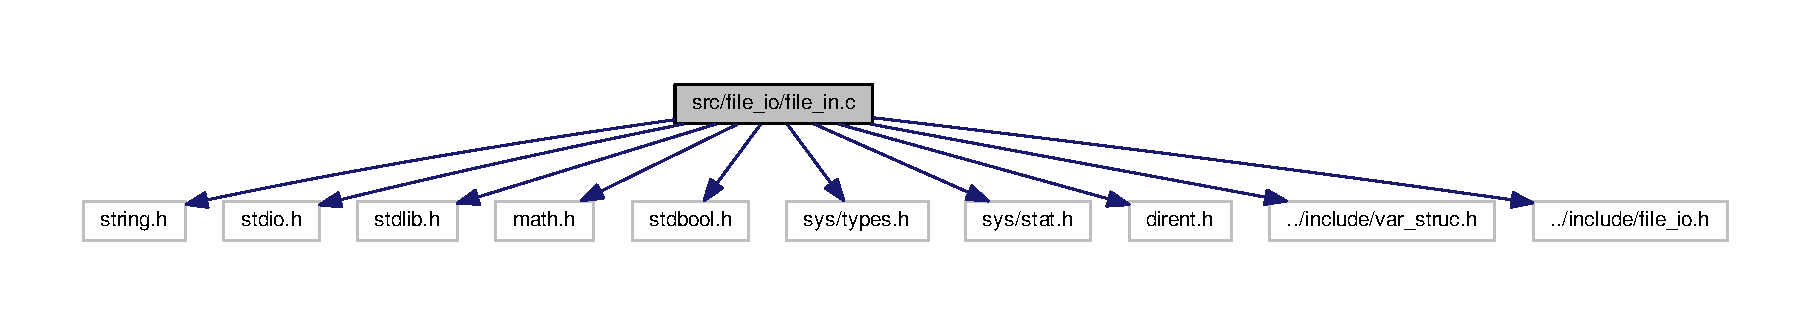
\includegraphics[width=350pt]{file__in_8c__incl}
\end{center}
\end{figure}
\subsection*{Functions}
\begin{DoxyCompactItemize}
\item 
int \hyperlink{file__in_8c_a99d4ed7b7cfd80a93fa861bd7d29e5cf}{file\+\_\+pre\+\_\+read} (F\+I\+LE $\ast$fp, int test\+\_\+lc)
\begin{DoxyCompactList}\small\item\em This function counts how many numbers are there in the initial data file. \end{DoxyCompactList}\item 
void {\bfseries initialize} (char $\ast$add, double $\ast$F)\hypertarget{file__in_8c_acb162616ea6c692468acaa3fe2ec79b2}{}\label{file__in_8c_acb162616ea6c692468acaa3fe2ec79b2}

\item 
void {\bfseries configurate} (char $\ast$add)\hypertarget{file__in_8c_a7d5de32dbd37998dfdf1feb389ece30e}{}\label{file__in_8c_a7d5de32dbd37998dfdf1feb389ece30e}

\item 
int {\bfseries config\+\_\+check} (void)\hypertarget{file__in_8c_a7cb5921c79aced1abe4d03ff43980d74}{}\label{file__in_8c_a7cb5921c79aced1abe4d03ff43980d74}

\end{DoxyCompactItemize}
\subsection*{Variables}
\begin{DoxyCompactItemize}
\item 
double {\bfseries config} \mbox{[}200\mbox{]}\hypertarget{file__in_8c_a6d077a61a7265ffdaed10089930f4926}{}\label{file__in_8c_a6d077a61a7265ffdaed10089930f4926}

\end{DoxyCompactItemize}


\subsection{Detailed Description}
This file is a collection of functions used to read files and check whether they are qualified. 

\begin{DoxyAuthor}{Author}
Du Zhifang, Lei Xin 
\end{DoxyAuthor}


\subsection{Function Documentation}
\index{file\+\_\+in.\+c@{file\+\_\+in.\+c}!file\+\_\+pre\+\_\+read@{file\+\_\+pre\+\_\+read}}
\index{file\+\_\+pre\+\_\+read@{file\+\_\+pre\+\_\+read}!file\+\_\+in.\+c@{file\+\_\+in.\+c}}
\subsubsection[{\texorpdfstring{file\+\_\+pre\+\_\+read(\+F\+I\+L\+E $\ast$fp, int test\+\_\+lc)}{file_pre_read(FILE *fp, int test_lc)}}]{\setlength{\rightskip}{0pt plus 5cm}int file\+\_\+pre\+\_\+read (
\begin{DoxyParamCaption}
\item[{F\+I\+LE $\ast$}]{fp, }
\item[{int}]{test\+\_\+lc}
\end{DoxyParamCaption}
)}\hypertarget{file__in_8c_a99d4ed7b7cfd80a93fa861bd7d29e5cf}{}\label{file__in_8c_a99d4ed7b7cfd80a93fa861bd7d29e5cf}


This function counts how many numbers are there in the initial data file. 

\begin{DoxyAuthor}{Author}
Du Zhifang, Lei Xin 
\end{DoxyAuthor}

\begin{DoxyParams}[1]{Parameters}
\mbox{\tt in}  & {\em fp} & The pointer of the file to read in. \\
\hline
\mbox{\tt in}  & {\em test\+\_\+lc} & Whether there is test for the range of data in the initial data file\+:
\begin{DoxyItemize}
\item 0 or 1 \+: no test,
\item 2 \+: 2-\/D test (CR separates row),
\item 3 \+: 3-\/D test (CR separates row, blank line separates column in x-\/y plane). 
\end{DoxyItemize}\\
\hline
\end{DoxyParams}
\begin{DoxyReturn}{Returns}
The number of the numbers in the initial data file. 
\end{DoxyReturn}

\begin{DoxyRetVals}{Return values}
{\em -\/1} & The given number of column is not coincided with that in the data file. \\
\hline
\end{DoxyRetVals}


Definition at line 33 of file file\+\_\+in.\+c.


%--- End generated contents ---

% Index
\backmatter
\newpage
\phantomsection
\clearemptydoublepage
\addcontentsline{toc}{chapter}{Index}
\printindex

\end{document}
